% !TeX program = xelatex
% ============================================================
% passport_ru.tex — Технический паспорт и сертификат калибровки
% ТГц перестраиваемый прецизионный аттенюатор (русскоязычная версия)
% ============================================================
\documentclass[11pt]{article}

\usepackage{myconfig}
\usepackage{booktabs}

% Русский язык уже подключён через babel в myconfig.sty — дополнительно не нужен
% (polyglossia несовместима с babel, не используем \setmainlanguage)

% Сквозная нумерация рисунков; подпись «Рисунок X.»
\counterwithout{figure}{section}
\captionsetup[figure]{name=Рисунок, labelsep=period, font=small,
                      labelfont=bf, justification=centering}


% Поля — максимально компактно, всё на 2 страницах
\geometry{
	left=1.4cm,
	right=1.4cm,
	top=1.0cm,
	bottom=1.0cm,
	headheight=0.4cm,
	footskip=0.4cm
}

% Уплотнение отступов вокруг плавающих объектов
\setlength{\floatsep}{4pt plus 2pt minus 1pt}
\setlength{\textfloatsep}{4pt plus 2pt minus 1pt}
\setlength{\intextsep}{4pt plus 2pt minus 1pt}
\setlength{\abovecaptionskip}{2pt plus 1pt minus 1pt}
\setlength{\belowcaptionskip}{2pt plus 1pt minus 1pt}

\singlespacing % одинарный межстрочный интервал

\begin{document}
	\pagestyle{empty} % без номеров страниц
	
	% ==========================================
	% СТРАНИЦА 1: ШАПКА И ХАРАКТЕРИСТИКИ
	% ==========================================
	\noindent
	\begin{minipage}[c]{0.26\textwidth}
		\vspace{0pt}
		
\includegraphics[width=\textwidth]{tydex_logo}
	\end{minipage}
	\hfill
	\begin{minipage}[c]{0.72\textwidth}
		\vspace{0pt}
		\raggedleft
		{\large\bfseries ООО «Тидекс»} \\
		{\small Отдел спектральных исследований} \\
		\vspace{0.2em}
		{\color{headerblue}\large\bfseries ТЕХНИЧЕСКИЙ ПАСПОРТ И СЕРТИФИКАТ КАЛИБРОВКИ} \\
		{\color{headerblue}\Large\bfseries ТГц Перестраиваемый Прецизионный Аттенюатор} \\
		{\small Модель: \textbf{ATT-11-16-CA85} \quad | \quad Заводской №: \textbf{\#02721}}
	\end{minipage}
	
	\vspace{0.3em}
	\hrule
	\vspace{0.3em}
	
	% Сноска-звёздочка
	\renewcommand{\thefootnote}{*}
	
	\noindent
	\begin{minipage}[t]{0.81\textwidth}
		\vspace{0pt}
		\noindent\textbf{1. Назначение и конструкция} \\
		Терагерцовый перестраиваемый прецизионный аттенюатор \mycode{ATT-11-16-CA85}
		(световой диаметр 85~мм) состоит из двух независимых проволочных поляризаторов.
		На Рисунке~1 приведена схема экспериментальной установки для измерения пропускания
		ТГц-излучения через решётки $P_1$ и $P_2$. Первый поляризатор ориентирован вдоль
		вектора поляризации падающего пучка (угол $\theta_1 = 0^\circ$), тогда как второй
		поворотный поляризатор (анализатор) поворачивается на угол $\theta_2 = \theta$.
		Вносимое ослабление регулируется изменением относительного угла
		$\theta = \theta_2 - \theta_1$. Прибор индивидуально откалиброван для диапазона
		частот от 0.05 до 2.0~ТГц ($\lambda > 150$~мкм).
	\end{minipage}
	\hfill
	\begin{minipage}[t]{0.16\textwidth}
		\vspace{0pt}
		\centering
		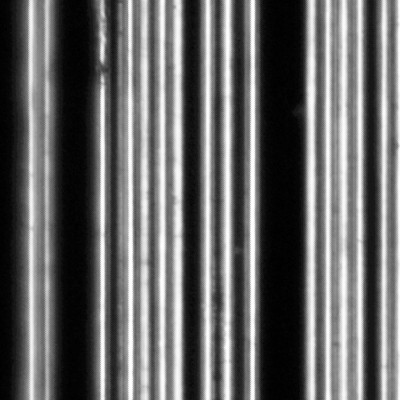
\includegraphics[width=\textwidth]{passport_microphoto}
		\par\vspace{1pt}
		{\small Фото структуры решётки}
	\end{minipage}
	
	\vspace{0.3em}
	
	\noindent\textbf{2. Технические и калибровочные характеристики}
	\begin{table}[H]
		\centering
		\small
		\begin{tabularx}{\textwidth}{lX}
			\toprule
			\textbf{Параметр} & \textbf{Значение / Техническая характеристика} \\
			\midrule
			Световой диаметр (диаметр держателя) & 85~мм \\
			Номинальный период решётки $P$ / диаметр проволоки $D$
				& $16.0$~мкм / $11.0$~мкм \\
			Измеренный геометрический период $P_{\text{geom}}$ (по фото)
				& $15.93 \pm 5.03$~мкм ($\pm 31.6\%$, класс качества «A») \\
			Калибровочный диапазон частот & 0.05 -- 2.0~ТГц \\
			\midrule
			\textbf{Эффективные параметры модели Бланко}
				& \textbf{Для расчёта калибровочных кривых (95\% ДИ):} \\
			Эффективный период решётки $P_{\text{eff}}$
				& $15.50 \pm 0.05$~мкм \\
			Эффективная ширина полосы $D_{\text{eff}}$\footnotemark[1]
				& $5.67 \pm 0.08$~мкм (среднее по ансамблю без дрейфа) \\
			Коэффициент омических потерь
				& $0.255 \pm 0.035$~дБ/ТГц$^{1.58}$ (степенной показатель $\gamma = 1.58$) \\
			Систематическое угловое смещение $\theta_{\text{offset}}$
				& $-0.45^\circ \pm 0.08^\circ$ (компенсация люфта вращателя) \\
			Ошибка аппроксимации модели (RMSE)\footnotemark[2]
				& $\pm 1.39$~дБ (динамический диапазон до $-45$~дБ) \\
			\bottomrule
		\end{tabularx}
	\end{table}
	\footnotetext[1]{\scriptsize Модель Бланко отображает цилиндрическую проволочную решётку
		на эквивалентную плоскую ленточную решётку. Круглая проволока номинальным диаметром
		$D = 11.0$~мкм взаимодействует с ТГц-излучением аналогично плоской металлической ленте
		шириной $d \approx D/2$, что даёт $D_{\text{eff}} \approx 5.67$~мкм. Коэффициент потерь
		включает степенную частотную зависимость $e^{-\alpha \nu^\gamma}$ с $\gamma = 1.58$
		для физического описания перехода от поглощения за счёт скин-эффекта ($\propto \nu^{0.5}$)
		к рэлеевскому рассеянию на микродефектах краёв проволоки ($\propto \nu^4$).
		См.: Blanco et al., \textit{Int. J. Infrared Millim. Waves}, vol.~7, no.~11, 1986.}
	\footnotetext[2]{\scriptsize Анализ 2D-невязок показывает, что ошибка модели обусловлена
		главным образом неучтёнными эффектами многократных межсеточных переотражений и
		дифракционного рассеяния на больших углах ($\theta > 50^\circ$), тогда как для малых
		углов ($\theta < 45^\circ$) RMSE локального фитинга менее $\pm 0.1$~дБ.}
	
	\vspace{-0.5em}
	
	\noindent\textbf{3. Схема эксперимента и методология} \\
	Калибровка аттенюатора проводилась на импульсном терагерцовом спектрометре
	(ТГц-ТДС) Menlo Tera~K8. Падающее излучение имело горизонтальную линейную
	поляризацию. Схема экспериментального измерения пропускания показана на Рисунке~1.
	
	\begin{figure}[H]
		\centering
		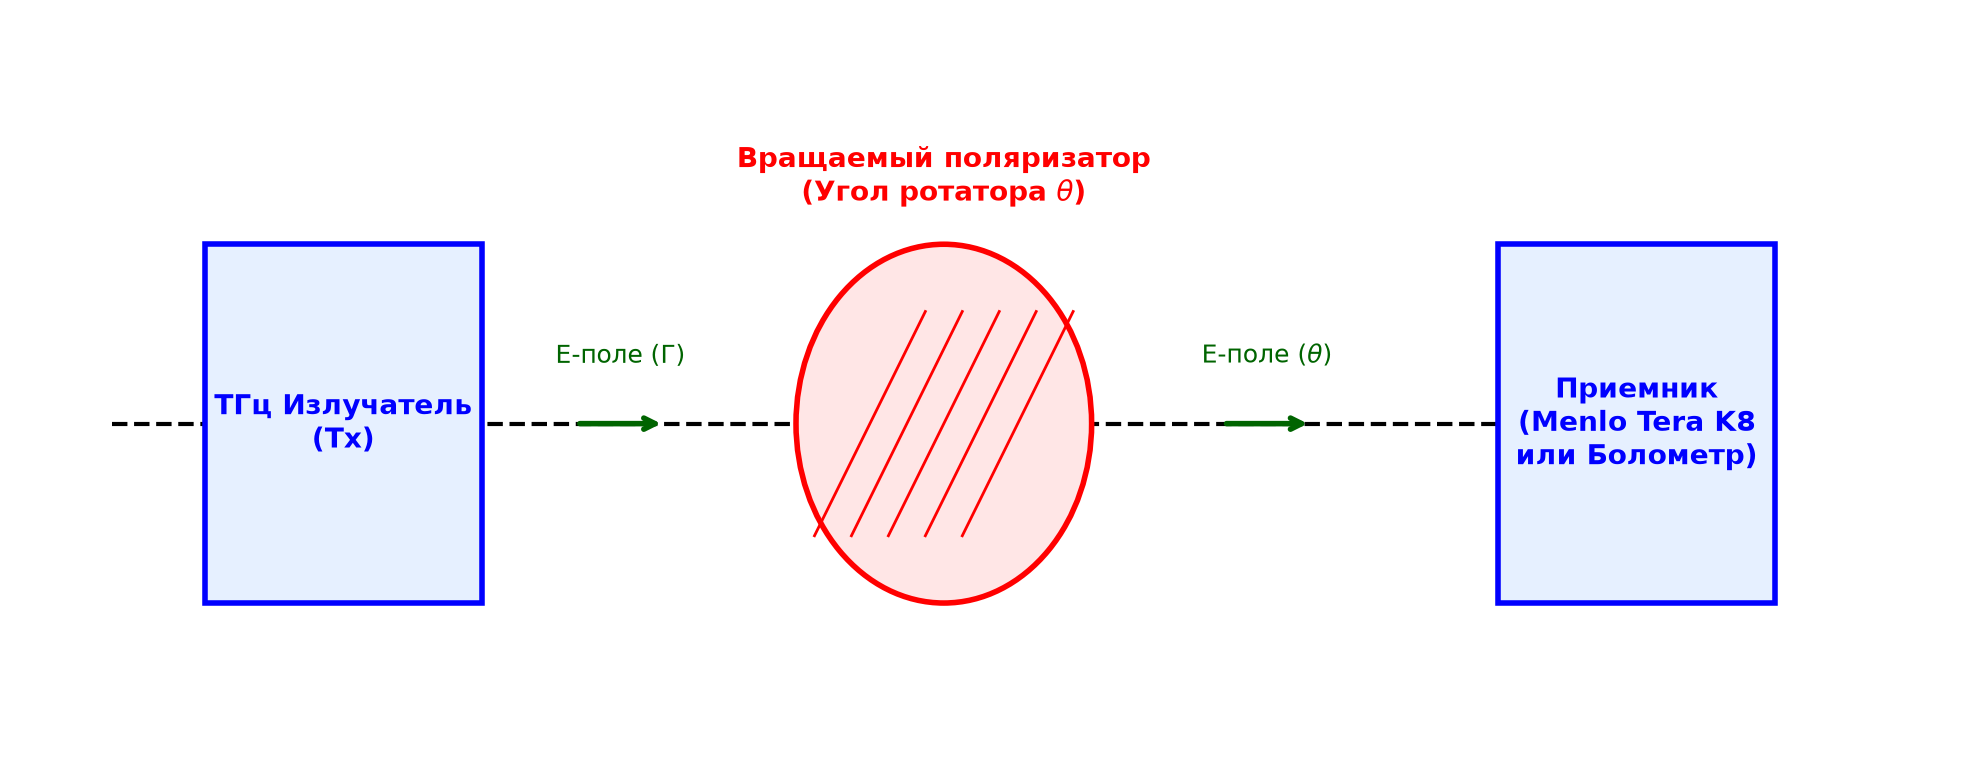
\includegraphics[width=0.60\textwidth]{fig0_1}
		\vspace{0.5em}
		\caption{Схема экспериментальной установки для калибровки аттенюатора
		         с углом поляризатора $\theta_1$ и углом анализатора $\theta_2$.}
		\label{fig:scheme}
	\end{figure}
	
	\newpage
	
	% ==========================================
	% СТРАНИЦА 2: КАЛИБРОВОЧНЫЕ КРИВЫЕ И АНАЛИЗ ПОГРЕШНОСТЕЙ
	% ==========================================
	\begin{center}
		{\color{headerblue}\large\bfseries КАЛИБРОВОЧНЫЕ КРИВЫЕ И ПОГРЕШНОСТИ АТТЕНЮАТОРА}
	\end{center}
	
	\vspace{0.2em}
	
	\noindent\textbf{4. Сценарии применения аттенюатора} \\
	В зависимости от типа приёмника коэффициент пропускания по мощности $T(\theta, \nu)$
	рассчитывается по модели Бланко\textsuperscript{*}, где
	$t_{\perp}(\nu) = t_{\perp,0}(\nu)\,e^{-\frac{1}{2}\alpha \nu^{\gamma}}$,
	$t_{\parallel}(\nu) = t_{\parallel,0}(\nu)\,e^{-\frac{1}{2}\alpha \nu^{\gamma}}$ ---
	скорректированные на потери комплексные амплитудные коэффициенты пропускания
	($t_{\perp,0},\,t_{\parallel,0}$ --- чистые электродинамические коэффициенты Бланко,
	$\alpha = 0.0587$~Нп/ТГц$^\gamma$, $\gamma = 1.58$),
	$\theta_{\text{offset}}$ --- систематический угловой сдвиг нуля шкалы,
	$T_{\text{noise}}$ --- шумовой пол:
	\begin{itemize}[leftmargin=0.6cm, itemsep=2pt, parsep=0pt, topsep=2pt]
		\item \textbf{Сценарий А} (ФПА Menlo Tera~K8 --- поляризационно-чувствительный приёмник): \\
		$T(\theta, \nu) = \left| t_{\perp}(\nu) \cos^2(\theta - \theta_{\text{offset}})
		                       + t_{\parallel}(\nu) \sin^2(\theta - \theta_{\text{offset}})
		                 \right|^2 + T_{\text{noise}}$
		\item \textbf{Сценарий Б} (Болометр / Ячейка Голея --- поляризационно-нечувствительный приёмник): \\
		$T(\theta, \nu) = |t_{\perp}(\nu)|^2 \cos^2(\theta - \theta_{\text{offset}})
		                + |t_{\parallel}(\nu)|^2 \sin^2(\theta - \theta_{\text{offset}})
		                + T_{\text{noise}}$
	\end{itemize}
	
	\vspace{0.3em}
	
	\noindent\textbf{5. Калибровочные кривые пропускания и ослабления} \\
	Для ручной регулировки ослабления используйте графические кривые на Рисунке~2.
	Чтобы задать требуемое ослабление $A$ (в дБ), найдите целевое значение на вертикальной
	шкале Рисунка~2 (справа или слева) и определите соответствующий угол поворота $\theta$.
	Левая панель показывает шкалу линейного пропускания для малых ослаблений
	($0^\circ$--$60^\circ$), правая панель --- шкалу в децибелах для глубоких ослаблений
	($30^\circ$--$90^\circ$). Экспериментальные точки Menlo на Рисунке~2 соответствуют
	измерениям по Сценарию~А и подтверждают высокую точность модели Бланко\textsuperscript{*}.
	
	\begin{figure}[H]
		\centering
		
\includegraphics[width=0.96\textwidth]{passport_calibration}
		\vspace{-0.5em}
		\caption{Калибровочные кривые: малые ослабления в линейном масштабе (слева)
		         и глубокие ослабления в масштабе дБ (справа). Правые оси --- альтернативные единицы.}
		\label{fig:calib}
	\end{figure}
	
	\vspace{-0.5em}
	
	\noindent
	\begin{minipage}[t]{0.56\textwidth}
		\vspace{0pt}
		\noindent\textbf{6. Анализ угловой погрешности позиционирования} \\
		Из-за тригонометрического характера закона Малюса чувствительность
		величины ослабления к угловой погрешности установки лимба $\Delta\theta$
		резко возрастает при углах $\theta > 70^\circ$. На Рисунке~3 показана
		погрешность ослабления $\Delta A$ для Сценария~А при аппаратных люфтах
		вращателя $\Delta\theta = 0.5^\circ$ и $1.0^\circ$.
		
		\vspace{0.4em}
		\noindent\textbf{7. Расчётное программное обеспечение и физические ограничения} \\
		В комплект поставки входит специализированное программное обеспечение для расчёта
		точного ослабления на любой частоте $\nu$ при любом угле $\theta$.
		Программа индивидуально откалибрована для данного конкретного прибора
		(заводской №~\#02721) с использованием эффективных параметров $P_{\text{eff}}$,
		$D_{\text{eff}}$ и $\theta_{\text{offset}}$. Программа распространяется по
		электронной почте. \\
		\textit{Ограничения}: на частотах ниже 10~ГГц ($\lambda > 3$~см) световой
		диаметр держателя (85~мм) становится соизмерим с длиной волны, что приводит
		к дифракционному рассеянию пучка на краях апертуры.
	\end{minipage}
	\hfill
	\begin{minipage}[t]{0.40\textwidth}
		\vspace{0pt}
		\centering
		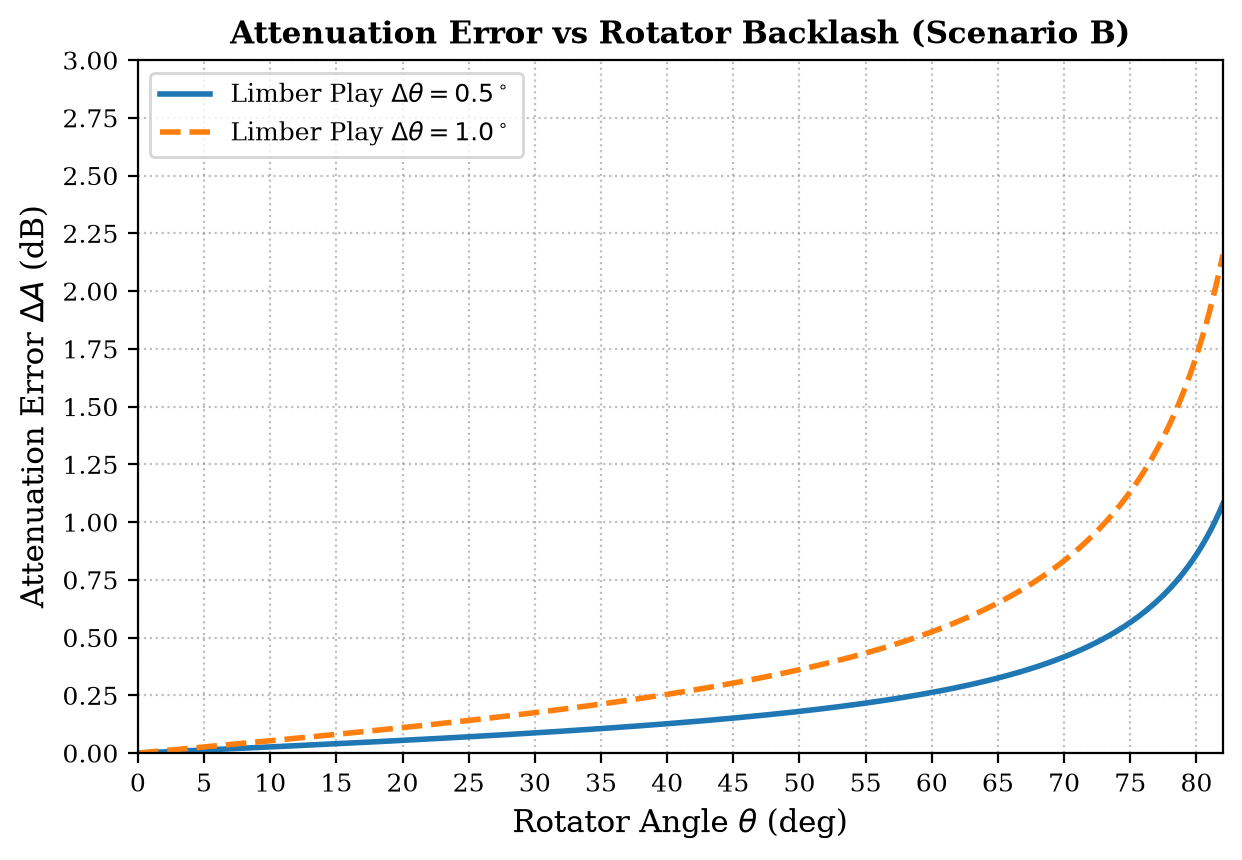
\includegraphics[width=\textwidth]{passport_error}
		\vspace{-0.6em}
		\captionof{figure}{Погрешность ослабления $\Delta A$ в зависимости от
		            угла вращения при люфтах $\Delta\theta = 0.5^\circ$ и $1.0^\circ$
		            (Сценарий~А).}
		\label{fig:error}
	\end{minipage}
	
	\vspace{0.6em}
	\hrule
	\vspace{0.4em}
	\begin{center}
		\small
		Дата калибровки: 29 июня 2026~г. \\
		\vspace{0.3em}
		\textbf{Отдел спектральных исследований, ООО «Тидекс»}
		\hfill
		\textbf{Подпись оператора: \underline{\hspace{4cm}}}
	\end{center}
	
\end{document}
